\documentclass[tikz,border=3mm]{standalone}
\usepackage[siunitx]{circuitikz}
\usetikzlibrary{calc,positioning,arrows.meta}

\begin{document}

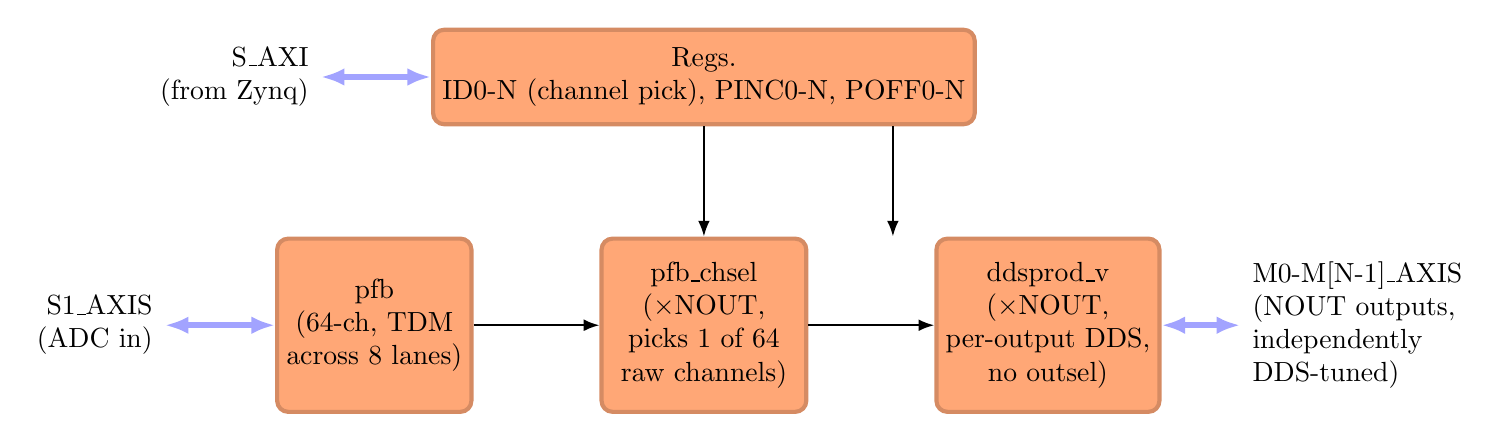
\begin{tikzpicture}
[box/.style={align=center, draw,rounded corners,minimum width=2cm,minimum height=1.2cm,draw={rgb,255:red,213; green,139; blue,99},fill={rgb,255:red,255; green,167; blue,118},line width=1.5pt},
arrow/.style={line width=2.2pt,draw={rgb,255:red,162; green,163; blue,255},{Latex[length=3mm]}-{Latex[length=3mm]}},
single arrow/.style={line width=0.8pt,-{Latex[length=2mm]}},
node distance=0.5cm]

% Channelizer.
\node[box,minimum height=2.2cm,minimum width=2.4cm] (pfb) {pfb\\(64-ch, TDM\\ across 8 lanes)};

% Per-output channel selector (pfb_chsel x NOUT).
\node[box,right=1.6cm of pfb,minimum height=2.2cm,minimum width=2.6cm] (chsel) {pfb\_chsel\\($\times$NOUT,\\ picks 1 of 64\\ raw channels)};

% Per-output DDS (ddsprod_v, one DDS per output now).
\node[box,right=1.6cm of chsel,minimum height=2.2cm,minimum width=2.6cm] (dds) {ddsprod\_v\\($\times$NOUT,\\ per-output DDS,\\ no outsel)};

% Regs.
\coordinate (temp) at ($(chsel.north)+(0,1.4)$);
\node[box,anchor=south,minimum width=6.5cm] (regs) at (temp) {Regs.\\ID0-N (channel pick), PINC0-N, POFF0-N};

% s1_axis: ADC in.
\draw[arrow] ($(pfb.west)+(-1.4,0)$) node[anchor=east,align=right] {S1\_AXIS\\(ADC in)} -- (pfb.west);

% s_axi.
\draw[arrow] ($(regs.west)+(-1.4,0)$) node[anchor=east,align=right] {S\_AXI\\(from Zynq)} -- (regs.west);

% pfb -> chsel.
\draw[single arrow] (pfb.east) -- (chsel.west);

% Regs -> chsel (ID0-N: which of the 64 channels).
\draw[single arrow] (regs.south) -- (regs.south |- chsel.north);

% Regs -> dds (PINC0-N/POFF0-N).
\coordinate (temp) at ($(regs.south)+(2.4,0)$);
\draw[single arrow] (temp) -- (temp |- dds.north);

% chsel -> dds.
\draw[single arrow] (chsel.east) -- (dds.west);

% outputs.
\draw[arrow] (dds.east) -- ++(1,0) node[anchor=west,align=left] {M0-M[N-1]\_AXIS\\(NOUT outputs,\\ independently\\ DDS-tuned)};

\end{tikzpicture}

\end{document}
